\subsection{Potenzreihen}

% \begin{align*}
%     &a_0 & + a_1 x^1 & + a_2 x^2 & + a_3 x^3 & + a_4 x^4 & + \cdots & + a_n x^n + & + \cdots \\
%     &a_0 (x-x_0)^0 & + a_1 (x-x_0)^1 & + a_2 (x-x_0)^2 & + a_3 (x-x_0)^3 & + a_4 (x-x_0) & + \cdots & + a_n (x-x_0)^n & + \cdots
% \end{align*}

\[
    \begin{array}{lll lll lll}
    &a_0 & + a_1\ x^1 & + a_2\ x^2 & + a_3\ x^3 & + a_4\ x^4 & + \cdots & + a_n\ x^n & + \cdots \\
    &a_0 (x-x_0)^0 & + a_1 (x-x_0)^1 & + a_2 (x-x_0)^2 & + a_3 (x-x_0)^3 & + a_4 (x-x_0) & + \cdots & + a_n (x-x_0)^n & + \cdots
    \end{array}    
\]

\begin{align*}
    \limtoinfty{n} \left| \frac{a_{n+1} \cdot x^{n+1}}{a_n \cdot x^n} \right| &< 1 \\
    \limtoinfty{n} \left| \frac{a_{n+1}}{a_n} \right| \cdot | x | &< 1 &&\left| \cdot \frac{1}{| x |} \right. \\
    \limtoinfty{n} \left| \frac{a_{n+1}}{a_n} \right| &< \frac{1}{| x |} \\
    | x | &< \underbrace{\limtoinfty{n} \left| \frac{a_n}{a_{n+1}} \right|}_{r_0} && r_0 = \text{Konvergenzradius} \\
    | x | &< r_0 \\
    \Rightarrow -r_0 < x < r_0
\end{align*}

\begin{figure}[H]
    \centering
    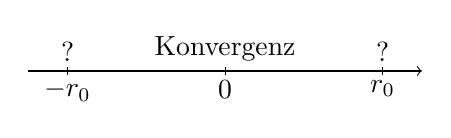
\begin{tikzpicture}
        \node[above] at (-2, 0) {?}; 
        \node[above] at (0, 0) {Konvergenz}; 
        \node[above] at (2, 0) {?};
        
        \node[below] at (-2, 0) {\( -r_0 \)}; 
        \node[below] at (0, 0) {\( 0 \)}; 
        \node[below] at (2, 0) {\( r_0 \)};

        \draw (-2, 0.05) -- (-2, -0.05); 
        \draw (0, 0.05) -- (0, -0.05); 
        \draw (2, 0.05) -- (2, -0.05); 
        \draw[->] (-2.5,0) -- (2.5,0);
    \end{tikzpicture}
\end{figure}

\paragraph{Beispiel}

\begin{align*}
    1)\qquad &1 + \frac{x}{1!} + \frac{x^2}{2!} + \frac{x^3}{3!} + \frac{x^4}{4!} + \cdots + \frac{x^n}{n!} + \cdots \\
    &r_0 = \limtoinfty{n} \left| \frac{a_n}{a_n + 1} \right| = \limtoinfty{n} \frac{\frac{1}{n!}}{\frac{1}{(n + 1)!}} = \limtoinfty{n} \frac{(n+1)!}{n!} = \limtoinfty{n} (n + 1) = \infty \\
    &\Rightarrow \text{konvergiert für alle } x \in \mathbb{R} \\
    2)\qquad &1 + \frac{x}{n} + \frac{x^2}{2} + \frac{x^3}{3} + \frac{x^4}{4} + \cdots + \frac{x^n}{n} \\
    &r_0 = \limtoinfty{n} \left| \frac{\frac{1}{n}}{\frac{1}{n + 1}} \right| = \limtoinfty{n} \frac{n + 1}{n} = \limtoinfty{n} \frac{1 + \frac{1}{n}}{1} = 1 \\
    &\text{die Reihe konvergiert für } |x| < r_0 = 1 \\
    &\text{für } x = -1 \Rightarrow \text{alternierene harmonische Reihe} \Rightarrow \text{konvergiert} \\
    &\text{für } x = 1 \Rightarrow \frac{1}{x} \Rightarrow \text{divergent} \\
    &-1 \leq x < 1 \\
    3)\qquad &1 - x + x^2 - x^3 + x^4 - x^5 \cdots = \frac{1}{1 + x} \qquad |x| < 1 \\
    &\entspricht q = -x \\
    &1 + q^1 + q^2 + q^3 + q^4 + q^5 + \cdots
\end{align*}

\begin{figure}[H]
    \centering
    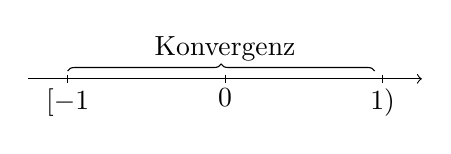
\begin{tikzpicture}
        \node[above] at (0, 0.1) {Konvergenz};
        \draw[decoration={brace}, decorate] (-2,0.1) -- (1.9,0.1);
        
        \node[below] at (-2, 0) {\( [-1 \)}; 
        \node[below] at (0, 0) {\( 0 \)}; 
        \node[below] at (2, 0) {\( 1) \)};

        \draw (-2, 0.05) -- (-2, -0.05); 
        \draw (0, 0.05) -- (0, -0.05); 
        \draw (2, 0.05) -- (2, -0.05); 
        \draw[->] (-2.5,0) -- (2.5,0);
    \end{tikzpicture}
    \caption{Grafische Darstellung von Beispiel 2}
\end{figure}
